\documentclass[12pt]{article}
\usepackage[utf8]{inputenc}
\usepackage[T1]{fontenc}
\usepackage{fixltx2e}
\usepackage{graphicx}
\usepackage{longtable}
\usepackage{float}
\usepackage{wrapfig}
\usepackage{soul}
\usepackage{textcomp}
\usepackage{marvosym}
\usepackage{xspace}
\usepackage{latexsym}
\usepackage{amssymb}
\usepackage[usenames,dvipsnames,svgnames,table]{xcolor}
\usepackage{hyperref}
\definecolor{darkblue}{rgb}{0.0,0.1,0.3}
\definecolor{darkgreen}{rgb}{0.0,0.35,0.15}
\definecolor{darkred}{rgb}{0.3,0.1,0.0}
\def\refColor{darkgreen}
\hypersetup{%
  colorlinks,
  linkcolor=\refColor,
  urlcolor=\refColor,
  anchorcolor=\refColor,
  citecolor=\refColor
}
\usepackage[hmargin={2.5cm,2cm}, vmargin=2.4cm]{geometry}
\tolerance=1000
\usepackage{listings}
\usepackage{math,ff++listings}
\usepackage{pgf}

\usepackage[noblocks]{authblk} % Authors
\setlength{\affilsep}{3em}

\providecommand{\alert}[1]{\textbf{#1}}
\providecommand{\structure}[1]{#1}

\newcommand{\FF}{\textit{FreeFem++}\xspace}
\newcommand{\FFcs}{\textit{FreeFem-cs}\xspace}
\renewcommand{\P}{\mathbb{P}_}
\newcommand{\R}{{\mathbb R}}

\newcounter{exercise}
\newenvironment{exercise}{%
  \stepcounter{exercise}
  \subsubsection*{Exercise~\theexercise.}}
{}

\title{Computer Practices: The Finite Element Method with \FF}

\author[$\dagger$]{Juan Vicente Gutiérrez Santacreu}
\author[$\ddagger$]{J. Rafael Rodríguez Galván}
\affil[$\dagger$]{Departamento de Matemática Aplicada I. Universidad de Sevilla. \texttt{juanvi@us.es}}
\affil[$\ddagger$]{Departamento de Matemáticas. Universidad de Cádiz. \texttt{rafael.rodriguez@uca.es}}

\date{
  \textsf{\textit{Doc-Course: ``Partial Differential Equations:
      Analysis, Numerics and Control''. Research Unit 3: Numerical
      Methods for PDEs}}
  \\[2em]
  \emph{April, 2018}
  \\[10em]
  
\includegraphics[width=0.07\textwidth]{./cc-by-sa.png}
  \\[1em]
  \begin{small} \scriptsize\em
    \href{http://creativecommons.org/licenses/by-sa/3.0/}{Creative
      Commons Attribution-Share\_Alike License, \\
      \scriptsize\url{http://creativecommons.org/licenses/by-sa/3.0/}}.
  \end{small}
}

% -----------------------------------
% Code listing style
% -----------------------------------
\definecolor{codegreen}{rgb}{0,0.6,0}
\definecolor{codegray}{rgb}{0.5,0.5,0.5}
\definecolor{codepurple}{rgb}{0.58,0,0.82}
\definecolor{backcolour}{rgb}{0.94,0.94,0.95}

\lstdefinestyle{mystyle}{
    % backgroundcolor=\color{backcolour},
    % commentstyle=\color{codegreen},
    % keywordstyle=\color{magenta},
    % numberstyle=\tiny\color{codegray},
    % stringstyle=\color{codepurple},
    basicstyle=\footnotesize\ttfamily,
    % basicstyle=\linespread{1.2}, % Line spacing
    % breakatwhitespace=false,
    % breaklines=true,
    % numbers=left,
    % numbersep=5pt,
    aboveskip=1.0em,
    belowskip=1.0em,
    language=freefem++
}
\lstset{style=mystyle}
% -----------------------------------


% -----------------------------------
\begin{document}
% -----------------------------------

\maketitle

%\large %%%%%%%%%%%%%%%%%%%%%%%%%%%%%%%%

\newpage
\setcounter{tocdepth}{2}
\tableofcontents
\vspace*{1cm}

\section{Introduction}
\label{sec:introduction}

\subsection{The \FF environment}
\label{sec:ff-environment}

\alert{\FF}\footnote{\url{http://www.freefem.org/ff++}} is a package
for \emph{numerical approximation of the solution of PDE} (partial
differential equations), both 2D and 3D, by means of the \textit{Finite
Element Method} (FEM). \FF is composed of:

\begin{itemize}

\item An interpreted \alert{programming Language}:
  \begin{itemize}
  \item Oriented to (1) fast specification of (linear and steady) PDE
    problems and (2) resolution of those problems, using the FEM.
  \item Allows easy implementation of complex problems (nonlinear,
    transient,...)
  \end{itemize}

\item An \alert{interpreter} for that language.
  \begin{itemize}

  \item Programs in FreeFem++ are interpreted (not compiled) at
    runtime. In this sense, FreeFem++ is a \textit{scripting} language
    (like Python, Matlab/Octave, Perl, and others).
  \item \FF is \alert{open source}/\alert{free software} (GNU GPL license).
  \item There are different versions: \texttt{FreFem++},
    \texttt{FreeFem++-nw}, \texttt{FreeFem++-mpi},\ldots{}
  \end{itemize} % ends low level
\end{itemize} % ends low level

\FF is mainly developed by \textbf{F. Hetch}.
\begin{center}
  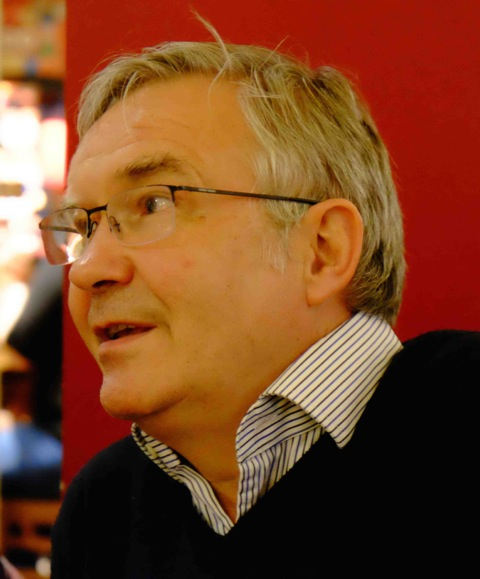
\includegraphics[width=0.3\linewidth]{./Hecht-portrait}
\end{center}

\subsection{What can you do with \FF?}
Let us present two examples, both of them related to the 2D steady
Stokes equations (which model viscous incompressible homogeneous fluxes):
\begin{equation*}
  \left\{
  \begin{aligned}
    -&\nu\Delta \mathbf{u}+ \nabla p= f
    \\
    &\nabla\cdot \mathbf{u}  = 0
    \\ & + \text{boundary conditions},
  \end{aligned}
  \right.
\end{equation*}
where the unknowns are $\mathbf{u}=(u,v):\Omega\to\R^2$ (velocity field of fluid)
and $p:\Omega\to\R$ pressure in each point of the domain.
\begin{itemize}
\item
  \href{https://www.youtube.com/watch?v=dn4UeMQDf9c&index=2&list=UUbv6VZ2UBw4iXCMR2L4G0zg&t=0s}{Video:
    Stokes/Navier-Stokes equations in Mediterranean sea.}
\item Why I like numerical simulation (as mathematician): it helps you
  to understand underlying maths
  (\href{https://www.youtube.com/watch?v=6x8KseewSrU&feature=youtu.be}{Video:
    instability of a numerical scheme}).
\end{itemize}


\subsection{Characteristics  of the \FF Language}
\begin{itemize}

\item Inspired by \alert{C/C++}.
  \begin{itemize}
  \item \emph{Similarities}: Syntax, strong typing\ldots{}
  \item \emph{Does not include}: Pointers, object orienting, \ldots{}
  \end{itemize}

\item \alert{Oriented} to numerical simulation using the finite element method.
  \alert{Capabilities}:
  \begin{itemize}
  \item Definition of the \textbf{geometry} of a problem and 2D/3D meshing.
    Although \FF is not a CAD/CAE environment and then, for complex
    geometries, it is necessary to use external tools.
  \item Variety of available \alert{finite elements}:
    $P_k$--Lagrange, $P_1$--bubble, $P_1$ discontinuous,
    Raviart-Thomas\ldots{}
  \item Flexibility for definition of problems which can be formulated
    in terms of PDE (and expressed by a \alert{variational formulation})
  \item Automation of the task of \textbf{assembling FEM matrices} (involved in
    underlying FEM linear systems) so that this task is \textit{transparent to the
    user}.
  \item Several algorithms for \alert{resolution of those linear
      systems}: LU, Cholesky, Crout, CG, GMRES, UMFPACK\ldots{}
  \item Facilities for \alert{post-processing} and \alert{2D/3D
      visualization}.  Although \FF no is not specialized in
    scientific visualization, it can be complemented with external
    tools for high-quality graphics.
  \item Other issues:
    \begin{itemize}
    \item Excellent documentation, including a \textbf{manual} (with a
      plenty of examples and tutorials):
      \url{http://www.freefem.org/ff++/ftp/freefem++doc.pdf}.
    \item (Matlab/Octave/Python/Fortran)--like matrix manipulation.
    \item Automatic interpolation between meshes, adaptive refinement,...
    \item Parallel (with MPI) version available
      (\texttt{FreeFem++-mpi}).
    \end{itemize}
  \end{itemize}

\end{itemize} % ends low level

\section{Installation and first steps}
\label{sec:inst-first-steps}

\FF is available for \href{http://www.freefem.org/}{download from its
  web page} or from the software center of some operative systems
(e.g. Debian or Ubuntu GNU/Linux).  Once installed, the \FF standard
distribution includes an interpreter for execution of code but no
editor or integrated environment (with editor, error feedback, syntax
highlighting, etc.). User is allowed to choose his/her
preferred editor between different possibilities, for instance (see
\FF manual for details):

\begin{itemize}
\item \textit{Crimson Editor} or \textit{Notepad++} on Windows,
\item \textit{Fraise editor} on MacOS.
\item \texttt{Emacs} on GNU/Linux, MacOS or Windows. Note that Emacs
  is a free/libre general-purpose (not only specialized in \FF)
  and powerful text editor.
\item \texttt{\FFcs} on GNU/Linux, MacOS or Windows. Note that \FFcs
  is integrated environment specialized in editing and post-processing
  \FF scripts.
\end{itemize}



% Anyway, for a first approach to \FF, we recommend \FFcs,
% \url{http://www.ann.jussieu.fr/~lehyaric/ffcs/}. \FFcs is an
% integrated environment providing \FF, and adequate editor and other
% characteristics. Of course, advanced users may prefer other options.

Here we review the configuration of the last two ones.

\subsection{Using \FF under Emacs}

Emacs can be installed form its
\href{https://www.gnu.org/software/emacs}{web page} of from the
software center of your operative system.
A \FF mode is available for Emacs, providing:
\begin{itemize}
\item Color-coded editor with automatic highlighting of \FF.
\item Integrated interface for running \FF scripts.
\item Tracking of compilation errors, linked back to the EDP source code.
\end{itemize}

For a \textbf{easy configuration} from scratch, it suffices to
download and unzip \textit{in your home user directory} the file
\texttt{freefem-emacs-basic-config.zip} which can be found in
\url{https://github.com/rrgalvan/freefem-mode/releases}.

For advanced configuration of \FF mode on Emacs, follow the
instructions from \url{https://github.com/rrgalvan/freefem-mode}.

\subsection{Using \FF under the integrated environment \FFcs}
\label{sec:freefem-CS}

\FFcs (\textit{CS} $\leftarrow$ Client/Server) is a multiple-platform
package which contains both \FF and an integrated environment for \FF
providing an intuitive interface. It adds to the goodies described for
Emacs the following characteristics:
\begin{itemize}
\item Integrated graphics area for 2d and 3d.
\item Online help including documentation in HTML.
\end{itemize}


\subsubsection{Installation}
For installation, you can get your preferred version from
the ``\textit{Download}'' link
(\url{http://www.ann.jussieu.fr/~lehyaric/ffcs/install.php}) and
follow the specific instructions for each  platform (which consist in
only a few steps). For instance:

\begin{itemize}
\item \textit{GNU/Linux} and \textit{MacOS}: Decompress the
  \texttt{.tgz} or the \texttt{.zip} file in your preferred location
  (for instance, in the desktop). Run the program \textit{FreeFem++-cs}.
\item \textit{Windows}: Execute the installation program and follow
  usual steps. Once installed, click on the \textit{FreeFem++-cs} icon
  and start using the application.
\end{itemize}

\subsection{First steps with \FF}

In the following exercise, we write a very simple FreeFem++ script
which plots a simple mesh in the unit square $[0,1]\times[0,1]$. This
mesh is defined by the subdivision of $[0,1]$ into to sub-intervals
(both in the $x$ axis in the $y$ axis).
\begin{exercise}
  Write the following code and run it. Test that a graphic
  is opened and a message is written in the bottom panel.
\begin{lstlisting}
mesh Th = square(2,2); // Declare a mesh object and build it
plot(Th);
cout << "This first mesh was properly drawn" << endl;
\end{lstlisting}
Former code may result quite familiar to C++ programmers. In
particular, notice that commentaries can be introduced by the
\texttt{//} operator and console output is produced by the familar C++
keywords \texttt{cout}, \texttt{endl} and the C++ streaming operator
\verb|<<|. On the other hand, \texttt{mesh} definition resembles C++
object constructors.

When running this example, a window will be opened showing the
mesh\footnote{Although in \FFcs, windows are opened in the right top
  panel}. Although this window contains no buttons or menus, it can be
controlled by the keyboard and by variables passed when
plotting. Press '\texttt{?}' key for help and for details see the \FF
manual and
\href{http://www.um.es/freefemv3/ff++/pmwiki.php?n=FFDoc.Plot}{'Plot'
  page in the FreeFem++ Wiki Manual}.

You can also notice that \FF produces a verbose
output\footnote{Which can be controlled by setting the variable
  \texttt{verb=n}, where \texttt{n} indicates the verbosity level. So
  that \texttt{verb=0} sets the lowest verbosity level.}, including
the whole code that was run and also some extra information and the
text which is streamed to the standard output using the keyword
'\texttt{cout}'.

\end{exercise}


\subsection{A First Realistic Example}

In this section we are going to solve a simple elliptic PDE problem by
means of the FEM method. More complex problems are left for further
sections.  Specifically, here we are going to solve the following
example (Poisson equation with homogeneous Dirichlet boundary
conditions) in a domain $\Omega\subset\Rset^2$ defined as the unit
circle:
\begin{equation*}
  \begin{cases}
    \text{Find } u:\overline\Omega \rightarrow \Rset
    \text{ such  that}
    \\\noalign{\medskip}
    \begin{aligned}
      -\Delta u &= f \quad\text{in } \Omega,
      \\
      u &= 0 \quad\text{on } \partial\Omega.
    \end{aligned}
  \end{cases}
\end{equation*}

For that purpose, we proceed as follows:
\begin{description}
\item[Step 1.] Express the problem in (discrete) variational formulation:
  \vspace{-1ex}
  \begin{equation*}
    \begin{cases}
      \text{Find } u:\overline\Omega \rightarrow \Rset
      \text{ such that }
      \\\noalign{\medskip}
      \begin{aligned}
        -\Delta u &= f \quad\text{in } \Omega,
        \\
        u &= 0 \quad\text{on } \partial\Omega.
      \end{aligned}
    \end{cases}
    \hspace{-1em}\leadsto\quad
    \begin{cases}
      \text{Find $u_h\in V_{h}$ such that}
      \\\noalign{\medskip}
      \begin{aligned}
        \int_\Omega \nabla u_h \cdot \nabla v_h = \int_\Omega f \cdot
        v_h,
        \quad \forall v_h\in V_{h}.
      \end{aligned}
    \end{cases}
  \end{equation*}

\item[Step 2.] Translate the variational formulation into \FF
  language.
  Supposing that the domain, $\Omega$, is given by the unit circle, we
  can write the following script :
\lstinputlisting[caption={First example: Poisson problem homogeneous Dirichlet conditions},label={first-example}]{code/poisson-first-example.edp}

\end{description}

This piece of code contains the fundamentals of FEM with \FF.
\begin{enumerate}
\item In lines 1 and 2 we define the circular domain. The technique
  consists of the parametrization of the boundary. Any domain with
  parametrizable boundary can be easily introduced in \FF.  For other
  domains, one has to use a specific tool for mesh construction.
\item In line 3 we define the FE (finite element) space,
  $\P1$--Lagrange in this case, and in line 4 we declare two variables
  in this space. We intend to use the first one, \texttt{u}, as the FE
  unknown (the \texttt{trial} function), and the second one, \texttt{v}
  as the \texttt{test} function.
\item In line 5 we define a function. Note that standard variables
  \texttt{x} and \texttt{y} are predefined and must not be declared.
\item In lines 6--9 we solve the variational problem. Note that those
  lines constitute a quasi-literal transcription of the variational
  problem formulated in \texttt{Step 1}. Some comments:
  \begin{enumerate}
  \item By default, PDE operators like gradient ($\nabla$) are not
    predefined (although they can be defined using macros, as we see
    in a further section). So one must use the operators \texttt{dx}
    (i.e. $\frac{\partial}{\partial x}$) and \texttt{dy}
    (i.e. $\frac{\partial}{\partial y}$). For 3D programs, also \texttt{dz}
    can be employed.
  \item Dirichlet conditions are imposed as the ``artificial'' sum of
    a term to the bilinear form.
  \end{enumerate}

\item Finally, in line 10 we plot the obtained solution. Scalar data
  (as is, in this case, $u$) is plotted by contour plots, while vector
  data is plotted as arrow field (for instance, the velocity unknown
  in the context of Stokes equations).
\end{enumerate}

\begin{exercise}
  Modify the previous example for solving Poisson equation in the unit
  square with $f=0$ and the following boundary conditions: $u=1$ on
  the top edge of the square, $u=0$ on bottom, left and right edges of
  the square.

  \emph{Hint: use ``mesh Th=square(n,n)'' to define a mesh with n
    subintervals in horizontal and vertical edges. Then boundary edges
    are labeled as 0 (bottom), 1 (right), 2 (top) and 3 (left)}.
\end{exercise}

\subsection{Saving to VTK for high-quality graphics}

Despite \FF includes powerful graphics, it also integrates nicely with
data analysis and visualization software
through the VTK file format.

VTK consists of an open source C++ library for visualization of
different types of data (scalar, vector, tensor, etc.). Last versions
of FreeFem++ include a module (called \texttt{iovtk}) which can be
loaded for use VTK. This way users can save any FE function to a
\texttt{.vtk} file and then employ any of the available advanced
applications for manipulation and visualization of the data contained
in that file. In section~\ref{sec:brief-intro-paraview} we delve into
one of those applications, called
Paraview\footnote{\url{http://www.paraview.org/}}.

The following code can be appended to the script above for saving the
solution, $u$, into a VTK file.

\begin{lstlisting}
load "iovtk";
savevtk("/tmp/output.vtk", Th, u, dataname="Temperature");
\end{lstlisting}

The module \texttt{iovtk} provides the function
\texttt{savevtk}. Their compulsory parameters are: (1) name of the
output VTK file, (2) name of the mesh, (3) FE function to be
saved. More than one function can be saved in the same file, as we
will see below. The last parameter is optional (but recommended) and
provides a name for each saved function. In this case, assuming that
the solution represents the equilibrium state of a heating experiment,
the only data set is called ``Temperature''. We can use this name to
access the data in the future (for instance using Paraview).


\section{Other Boundary Conditions}
\label{sec:complex-problems}

In this section we go beyond the Poisson problem and generalize it for different boundary conditions:
\begin{enumerate}
\item Neumann boundary conditions.
\item Robin boundary conditions.
\end{enumerate}

\subsection{Poisson Problem With Mixed Neumann/Dirichlet Boundary Conditions}
\label{sec:poisson-problem-with-mixed-bc}

Let us consider the following problem: given
\begin{itemize}
\item $\Omega\subset\R^2$, with smooth piecewise boundary, divided into
  two non-empty subsets:
  $\partial\Omega=\Gamma_D\cup\Gamma_N$,
\item $\nu>0$, $f: \Omega \to \Rset$, $g_D:\Gamma_D\to\Rset$ and
$g_N:\Gamma_N\to\Rset$,
\end{itemize}
find $u:\overline\Omega \rightarrow \R$ such that:
\begin{equation}
  \label{eq:poisson-mixto}
  \begin{cases}
    \begin{aligned}
      -\nu\Delta u &= f \quad \text{ in } \Omega, \\
      u &= g_D \quad \text{ on } \Gamma_D, \\
      \frac{\partial u}{\partial n} &= g_N \quad \text{ on } \Gamma_N.
    \end{aligned}
  \end{cases}
\end{equation}
Notice that we consider a Dirichlet b.c. in $\Gamma_D$ and
a Neumann b.c on $\Gamma_N$. Remember that last condition means, means
$\nabla u \cdot n=g_N$, where $n$ is the exterior normal vector.

\begin{itemize}
\item The theory for \textbf{non-homogeneous Dirichlet} conditions,
  $u|_{\Gamma_D}=g_D$, is based on writing the solution as
  $$
  u = u_0 + u_D,
  $$
  where $u_0$ is a solution of the homogeneous problem
  ($u|_{\Gamma_D}=0$) and $u_D$ verifies $u|_{\Gamma_D}=g_D$.
  Algorithms for implementing generic Dirichlet conditions requires
  some kind of computing technique\footnote{In practice, for Dirichlet
    conditions one proceed as follows:
  \begin{enumerate}
  \item Build the FE linear system $Ax=b$, where $A$ comes from a
    bilinear form, $a(\cdot,\cdot)$ and $b$ comes from the linear form,
    $L(\cdot)$. Both of $A$ and $b$ are, typically constructed by
    quadrature formulae in triangles.
  \item Select the rows of $A$ and $b$ which correspond to equations
    for degrees of freedom on $\Gamma_D$. Then modify them,
    imposing explicitly the value of $u$ on those degrees of
    freedom. Typically, just the diagonal element and the RHS (containing
    the boundary value) are multiplied by a Huge number.
  \end{enumerate}
} which is automatized by \FF (just the operator '\texttt{on(\ )}' is used
as in previous examples) and then we are not going deeper.

  % writing the variational formulation, we  assume the homogeneous
  % Dirichlet condition
  % $$u=0 \text{ on } \Gamma_N,$$
  % and imposing later $u=g_D$ on $\Gamma_D$.
\item Moreover \textbf{Neumann boundary conditions} appear in a natural way in the
  variational formulation. Specifically, when the Green formula
  (integration by parts) is applied, one gets the following problem:
  \begin{equation*}
      \begin{cases}
      \text{Find $u_h\in V_{h}$ such that}
      \\\noalign{\medskip}
      \begin{aligned}
        \nu\int_\Omega \nabla u_h \cdot \nabla v_h = \int_\Omega f\, v_h
        + \nu\int_{\Gamma_N} g_N\, v_h
        \quad\text{for all } v_h\in V_{h},
      \end{aligned}
    \end{cases}
  \end{equation*}
  where for a fixed polynomial degree $k\in\mathbb{N}$,
  $$V_h=\big\{v_h\in C^0(\Omega) \text{ such that }
  v_h|_T \in \mathbb{P}_k[x] \ \forall T\in \mathcal{T}_h \text{ and } v_h|_{\Gamma_D}=0\big\}.
  $$
  \end{itemize}

  Here we show a FreeFem++ program for the Poisson problem presented
  above.  Here we use the keyword \texttt{problem} for defining the
  variational problem, which is solved later (instead of
  \texttt{solve}, which was used in Example~\ref{first-example} for
  defining and solving the problem).

\lstinputlisting[
caption={Poisson problem with mixed Dirichlet/Neumann boundary conditions},
label={dirich-neumann}
]{code/poisson-Dirich-Neumann.edp}

\section{Delving into the FreeFem++ language}
\label{sec:delv-into-freef}

\subsection{Data Types, Arrays and Matrices}
\label{sec:data-types-arrays}

Fundamental data types are similar to C++. But some fundamental types of C++ are not present in FreeFem++ (and vice versa) for instance:
\lstinputlisting[
caption={FreeFem++ fundamental data types and operations},
]{code/variables.edp}

\subsection{Linear System Associated to FEM}
\label{part:line-syst-assoc}

The keyword \texttt{varf} can be used in \FF to store the matrix and
vector related to a variational formulation. Then the operator
\verb|^-1*| can be used to solve the associated linear system.  The
advantage of using the \texttt{varf} approach is that, if used
properly, it is faster that \texttt{solve} or \texttt{problem} (about
4 times faster, according to \FF documentation).

The following script uses \texttt{varf} for solving Example~\ref{dirich-neumann}.

\lstinputlisting[
caption={Linear System Associated to Variational Formulation},
]{code/poisson-varf.edp}

\begin{exercise}
  Compare computing time of \texttt{problem} and \texttt{varf}
  approaches for solving the Poisson problem with Dirichlet
  conditions.  Search FreeFem++ documentation for find a function
  which can be utilized for calculation of the computing
  time. \textit{Hint: use the function \texttt{clock(\ )} for getting
    current time, then compute time difference.}
\end{exercise}

\section{Solving Evolution Equations}
\label{sec:solv-evol-equat}

\subsection{The Implicit Euler Method for the Heat Equation}
\label{sec:heat-equation}
\newcommand{\deltaT}{\Delta t}

Former examples were steady, namely time independent. In this section
we are going to solve the following transient problem (heat equation
with mixed Dirichlet+Neumann boundary conditions). Of course, although
the solution is going to be called ``temperatura'', it is applied to
any parabolic diffusive law (e.g. in biological models). The problem
reads: find $u=u(x,t)$ such that
\begin{equation}
  \label{eq:heat equation}
  \left\{
    \begin{aligned}
      \frac{\partial u}{\partial t} -\nu\Delta u &= f \quad \text{ in } \Omega, \\
      u(0)&=u_0 \text{ in } \Omega, \\
      u &= g_D \quad \text{ on } \Gamma_D, \\
      \frac{\partial u}{\partial n} &= g_N \quad \text{ on } \Gamma_N.
    \end{aligned}
    \right.
\end{equation}
Here:
\begin{itemize}
\item $x\in\Omega\subset\R^2$, with smooth piecewise boundary,  $\partial\Omega=\Gamma_D\cup\Gamma_N$
\item $t\in [0,T]$, where $T>0$ is the final time
\item $u_0$: $\Omega\to\R$: temperature at initial time.
\item $\nu>0$, $f:\Omega\times(0,T)\to\R$ (heat source in the domain),
  $g_D:\Gamma_D\times(0,T)\to\R$ (heat source on Dirichlet boundary $\Gamma_D$),
  $g_N:\Gamma_N\times(0,T)\to\R$ (heat source on Neumann boundary $\Gamma_N$).
\end{itemize}

For time discretization, we fix $n\in\Nset$ and consider the
following $n+1$ time instants in $[0,T]$:
$$t_m= \deltaT\cdot k, \ m=0, ..., N$$
where $\deltaT=T/N$ is the time step.

The \textit{Implicit Euler} method for~(\ref{eq:heat equation}) can be
written as follows:
% \begin{align*}
%   \frac{\partial u}{\partial t}  \approx \frac{u^{k+1}-u^k}{\deltaT} \\
%   \Delta u \approx \Delta u^{k+1}
% \end{align*}
Given $u^0_h=u_0$, for each $m=0,...,N-1$, find $u^{m+1}_h\in U_h$ (space
defined in section~\ref{sec:poisson-problem-with-mixed-bc}) such that:
\begin{equation}
  \label{eq:euler-implicit-heat-equation}
  \left\{
    \begin{aligned}
      \frac{u^{m+1}_h-u^m_h}{\deltaT} -\nu\Delta u^{m+1}_h &= f^{m+1}_h \quad \text{ in } \Omega, \\
      u^{m+1}_h &= g_D^{m+1} \quad \text{ on } \Gamma_D, \\
      \frac{\partial u^{m+1}_h}{\partial n} &= g_N^{m+1} \quad \text{ on } \Gamma_N.
    \end{aligned}
    \right.
\end{equation}
Former problem can be written in variational formulation as follows:
\begin{equation*}
  a(u^{m+1}_h,v_h) = b(v_h) \quad \forall v_h\in U_h,
\end{equation*}
where
\begin{equation*}
    \begin{aligned}
      a(u,v)&=\frac{1}{\deltaT} \int_\Omega u^{m+1} v + \nu\int_\Omega \nabla
      u^{m+1} \cdot \nabla v,
      \\
      b(v)  &= \int_\Omega f \cdot v
      +\frac{1}{\deltaT} \int_\Omega  u^{m} v
      +\int{\Gamma_N} \nu\int_\Omega g1 v.
    \end{aligned}
\end{equation*}
% \begin{equation}
%   \begin{cases}
%     \frac{\partial u}{\partial t} -\nu\Delta u = f \text{ in } \Omega\times(0,T), \\
%     u = g_D \text{ on } \Gamma_D\times(0,T), \\
%     u = g_N \text{ on } \Gamma_N\times(0,T), \\
%   \end{cases}
% \end{equation}



\subsubsection{\FF program}
For instance, the following script shows the resolution of heat
equation by implicit Euler time
scheme~(\ref{eq:euler-implicit-heat-equation}), for the following data:
\begin{itemize}
\item Domain $\Omega$: unit circle.  $\partial\Omega$ is split
  into two boundaries: $\Gamma_D$ is defined by angle in $(0,\pi/4)$
  while $\Gamma_D$ is defined by angle in $(\pi/4,2\pi)$. Space
  discretization is defined by $100$ sub-intervals approximating
  $\partial\Omega$.
\item Time interval: $[0,T]=[0,1]$, with time step $\delta_T=1/100$.
\item Initial boundary condition: $u(x,0)=0$ in $\Omega$. Dirichlet
  boundary condition: $g_D(x,t)= 100-100/(t+1)$ on
  $\Gamma_D\times (0,T)$. Neumann boundary condition: $g_N(x,t)=0$ on
  $\Gamma_N\times (0,T)$.
\item $f=0$, viscosity parameter $\nu=1$.
\end{itemize}

\lstinputlisting[
caption={Heat Equation},
label={lst:heat-ei}
]
{code/heat-EI.edp}

\appendix

\section{Poisson Problem With Robin Boundary Conditions}

Let us consider the following PDE problem, which generalizes~(\ref{eq:poisson-mixto}):
\begin{equation}
  \label{eq:poisson-robin}
  \begin{cases}
    \begin{aligned}
      -\nu\Delta u &= f \quad \text{ in } \Omega, \\
      u &= g_D \quad \text{ on } \Gamma_D, \\
      au + b \frac{\partial u}{\partial n} &= g_N \quad \text{ on } \Gamma_N,
    \end{aligned}
  \end{cases}
\end{equation}
where $a,b\in\Rset$. For $a,b\neq 0$, the third equation
in~(\ref{eq:poisson-robin}) is termed a \textit{Robin boundary
  condition}.

Integration by parts one can obtain the following variational formulation:
\begin{equation*}
  \begin{cases}
    \text{Find $u_h\in U_{h}$ such that}
    \\\noalign{\medskip}
    \begin{aligned}
      \nu\int_\Omega \nabla u_h \cdot \nabla v_h
      + \nu\frac a b \int_{\Gamma_N} u v
      = \int_\Omega f\, v_h
      + \nu \frac 1b \int_{\Gamma_N} g_N\, v_h
      \quad\text{for each } v_h\in U_{h},
    \end{aligned}
  \end{cases}
\end{equation*}
being $U_h$ defined as above.

\begin{exercise}
  Develop a FreeFem++ script for the finite element approximation of
  the solution of the problem presented above. For instance, use
  $a=1, b=1$ and the same domain and data as in
  \lstlistingname~\ref{dirich-neumann}.
\end{exercise}

\section{The Stokes equations}
\label{sec:stokes}

The Stokes equations can be considered as the linear steady version of
Navier-Stokes equations (which describe the behaviour of a newtoninan
fluid as atmosphere, ocean, flux around vehicles, etc.
\begin{equation*}
  \left\{
  \begin{aligned}
    -\nu\Delta \mathbf{u}+ \nabla p &= f
    \\
    \nabla\cdot \mathbf{u} & = 0
    \\ & + \text{boundary conditions},
  \end{aligned}
  \right.
\end{equation*}
where the unknowns are: $\mathbf{u}=(u,v):\Omega\to\R$ (velocity field
of fluid) and $p:\Omega\to\R$ pressure in each point of the domain.
Thus the first equation must be understood in vectorial way,
specifically, in the 2D case:
\begin{align*}
  \Delta u + \partial_x p &= f_1, \\
  \Delta v + \partial_y p &= f_2,
\end{align*}
where  $f=(f_1,f_2)$.

In this section we show a usual test for the Stokes 2D simultion,
which is know as \textbf{cavity test}. This test is usually run in a
rectangular domain but, in this case, with the purpose of illustrate
the construction in \FF of complex parametric geometries, we have
introduced some holes in the rectangular domain. They are defined by
parametric figures which are known as
conchoids\footnote{\url{http://en.wikipedia.org/wiki/Conchoid_\%28mathematics\%29}}.

Homogeneous Dirichlet b.c., $(u,v)=(0,0)$, are imposed for
$\mathbf{u}$ on the whole boundary excepting the top line, where we
fix $(u,v)=(1,0)$  (positive horizontal velocity). We use the stable
FE combination  $\P2/\P1$ (polynomials with degree $2$ for velocity
and degree $1$ for pressure).



\subsection{\FF Programming of 2D Stokes System}

\lstset{language=freefem++}
\begin{lstlisting} [caption={Steady Stokes System}]
// 2D Stokes equations
// Cavity test in a domain with some parametric holes

//,------------------------------------------------
//| STEP 1. Defining the domain and meshing it
//`------------------------------------------------

// Macro for the 2D boundary defining a hole. They are parametric
// curves called "conchoids". In the macro:
// n = number of 'petals', P = center of the hole
int NMAX=20;
macro conchoid(name, n, P, thelabel)
 name(i=0,NMAX) {
    real a=1.0, b=2.0;
    real theta = i*2*pi/NMAX;
    real rho = a * cos(n*theta)+b;
    x = P[0] + rho*cos(theta);
    y = P[1] + rho*sin(theta);
    label = thelabel;
} // EOM

// Definition of some conchoids
border conchoid(c2,2,[0,0]   ,0);
border conchoid(c3,3,[-10,0] ,0);
border conchoid(c4,4,[0,0]   ,0);
border conchoid(c5,5,[10,0]  ,0);
border conchoid(c6,6,[0,0]   ,0);
border conchoid(c7,7,[0,0]   ,0);

// External rectangle
real xcoor = 15, ycoor = 5;
border lx1(k=-xcoor,xcoor) { x=k; y=-ycoor; label=1; }
border lx2(k=-xcoor,xcoor) { x=k; y=+ycoor; label=3; }
border ly1(k=-ycoor,ycoor) { x=-xcoor; y=k; label=2; }
border ly2(k=-ycoor,ycoor) { x=+xcoor; y=k; label=2; }

int nx=40, ny=20, nc=50;
mesh Th = buildmesh( ly1(-ny)+lx1(nx)+ly2(ny)+lx2(-nx)
    + c3(-nc) + c4(-nc) + c5(-nc) );

//,--------------------------------------------------------
//| STEP 2. Resolution of Stokes problem in previous domain
//`--------------------------------------------------------

fespace Uh(Th,P2); Uh u,v,uu,vv;  // Velocity functions
fespace Ph(Th,P1); Ph p,pp;       // Pressure functions

real upperVelocity=1;

macro grad(u) [dx(u), dy(u)] // end of macro

// Definition of Stokes problem

problem stokes2d( [u,v,p], [uu,vv,pp], solver=LU) =
    int2d(Th)(
	grad(u)'*grad(uu) + grad(v)'*grad(vv)
	+ grad(p)'*[uu,vv] + pp*(dx(u)+dy(v)) //'
	- 1e-10*p*pp )
  + on(0,1,2,u=0,v=0) + on(3,u=upperVelocity,v=0);

stokes2d;  // Resolution of Stokes problem

// Save to VTK (for high quality plotting)
load "iovtk";
savevtk("/tmp/stokes.vtk", Th, [u,v,0], p);
\end{lstlisting}


\section{Paraview}
\label{sec:brief-intro-paraview}

ParaView is an open source multiple-platform application for
interactive, scientific visualization. It was developed to analyze
extremely large datasets using distributed memory computing
resources. It can be run on supercomputers to analyze datasets of
terascale as well as on laptops for smaller data.

For visualization of data, that lives in a mesh where the simulation
was performed, there are basically three steps:
\begin{enumerate}
\item \textit{Reading} data into Paraview (from a VTK file)
\item \textit{Filtering}, that is applying one or more filters in order to
  generate, extract or derive features from data.
\item \textit{Rendering} an image from the data and adjusting the
  viewing parameters for improve the final visualization.
\end{enumerate}

This tree steps are controlled through a panel in the right, called
\texttt{Pipeline browser}. The pipeline concept consists on a chain of
modules, starting from the data stored in a file. Each
of them takes in some data, operates on it and presents the result in
a dataset.
From the Paraview users guide:
\begin{quote}\small
  ``Reading data into ParaView is often as simple as selecting
  \texttt{Open} from the \textit{File} menu, and then clicking the
  glowing \textit{Accept} button on the reader's \textit{Object
    Inspector} tab. ParaView comes with support for a large number of
  file formats, and its modular architecture makes it possible to add
  new file readers.  Once a file is read, ParaView automatically
  renders it in a view. In ParaView, a view is simply a window that
  shows data. There are different types of views, ranging from
  qualitative computer graphics rendering of the data to quantitative
  spreadsheet presentations of the data values as text. ParaView picks
  a suitable view type for your data automatically, but you are free
  to change the view type, modify the rendering parameters of the data
  in the view, and even create new views simultaneously as you see fit
  to better understand what you have read in. Additionally, high-level
  meta information about the data including names, types and ranges of
  arrays, temporal ranges, memory size and geometric extent can be
  found in the \textit{Information} tab.''
\end{quote}
Advanced data processing can be done using the Python Programmable
filter with VTK, NumPy, SciPy and other Python modules.

\bigskip

For further details:
\begin{enumerate}
\item Video showing how to use FreeFem++ and Paraview for
  visualization of 2D and 3D cavity tests for the Stokes Equations
  (partially in
  spanish). \url{https://www.youtube.com/watch?v=wChDeo2A03E}
\item Paraview Wikipedia page (in which this appendix is
  based). \url{http://en.wikipedia.org/wiki/ParaView}.
\item Resources in the web, for instance
  \url{http://vis.lbl.gov/NERSC/Software/paraview/docs/ParaView.pdf}.
\item The paraview users guide (how to unleash the beast!)
  \url{http://denali.princeton.edu/Paraview/ParaViewUsersGuide.v3.14.pdf}
\end{enumerate}
\end{document}

%%% Local Variables:
%%% mode: latex
%%% TeX-master: t
%%% ispell-local-dictionary: "english"
%%% End:
